\documentclass[CMPE]{KGCOEReport}

\usepackage{graphicx}
\usepackage{float}
\newcommand{\classCode}{CMPE 160}  
\newcommand{\name}{Christopher Larson}
\newcommand{\LabSectionNum}{L3}
\newcommand{\LabInstructor}{Mr.\ Dominguez}	
\newcommand{\TAs}{TA Andrew Ramsey \\ TA Matthew Millar \\ TA Madeline Mooney}
\newcommand{\LectureSectionNum}{01}
\newcommand{\LectureInstructor}{Professor Beato}
\newcommand{\exerciseNumber}{04}
\newcommand{\exerciseDescription}{Analysis and Simulation of Sequential Circuits }
\newcommand{\dateDone}{7 March 2018}
\newcommand{\dateSubmitted}{21 March 2018}

\begin{document}
\maketitle

\section*{Abstract}
The objedctive of this exercise was to analyze and simulate sequential circuit-4 bit shift register. The exercise was helpful in the understanding of the design and operation of sequential circuits. A 4-bit shift register was designed and tested against a testbench to ensure the correctness of the design. The minimum clock period and maximum clock frequency were also recorded. A 4-bit register was also designed but the AND-OR gates network was replaced with tri-state buffers.

\section*{Design Methodology}
The schematic diagram that was designed represented a 4-bit shift register, as shown in Figure 1.

\begin{figure}[H]
	\centering
	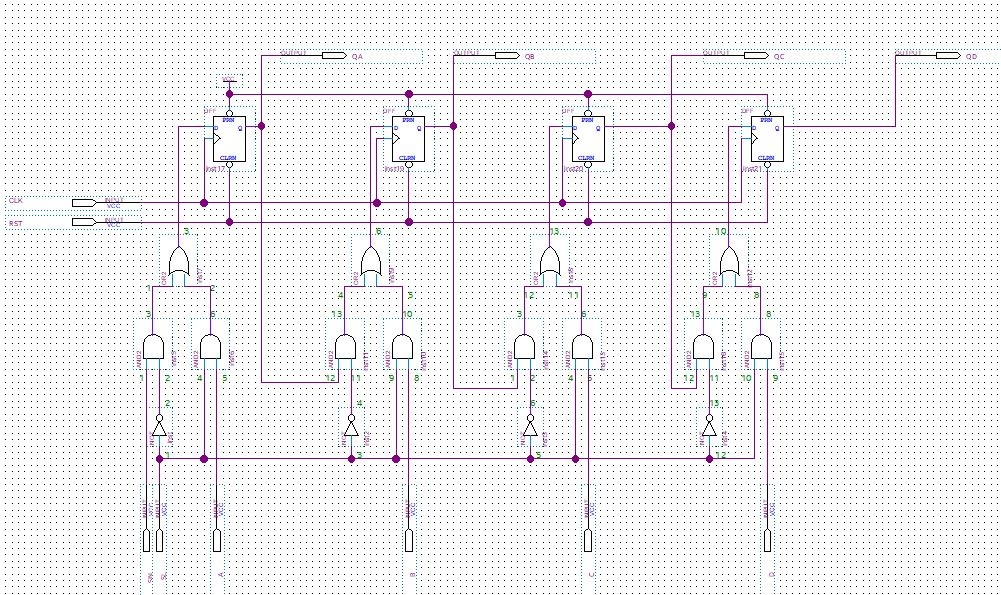
\includegraphics[width=\textwidth]{Circuit1.png}
	\caption{4-bit shift register}
	\label{fig: Figure 1}
\end{figure}

Figure 1 shows the diagram of a 4-bit shift register that was used to create the waveform. The 4-bit shift register with tri-state buffers was also desgined and tested against a testbench as well as the waveform was compared to the first waveform to ensure that the two diagrams worked the same. The 4-bit shift register diagram is shown in Figure 2.

\begin{figure}[H]
	\centering
	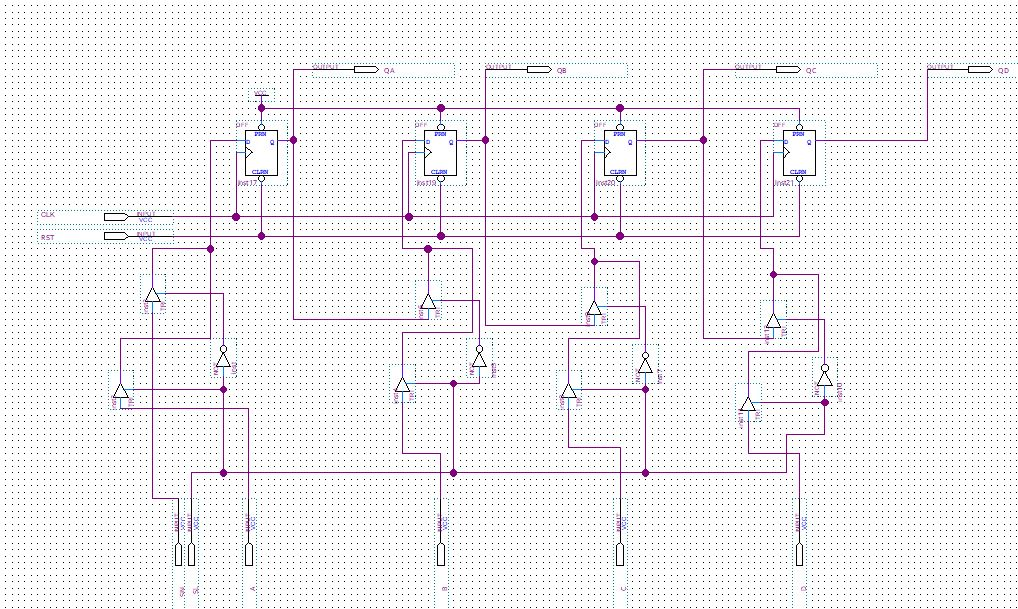
\includegraphics[width=\textwidth]{Circuit2.png}
	\caption{4-bit shift register with tri-state buffers}
	\label{fig: Figure 2}
\end{figure}

\section*{Results and Analysis} 
The waveform for both the 4-bit shift register and 4-bit register with tri-state buuffers is shown below. There is only one waveform because the two waveforms were the exact same since the two shift registers are functionally the same. The two waveforms were compared to each other to confirm the correctness of the diagrams. 

\begin{figure}[H]
	\centering
	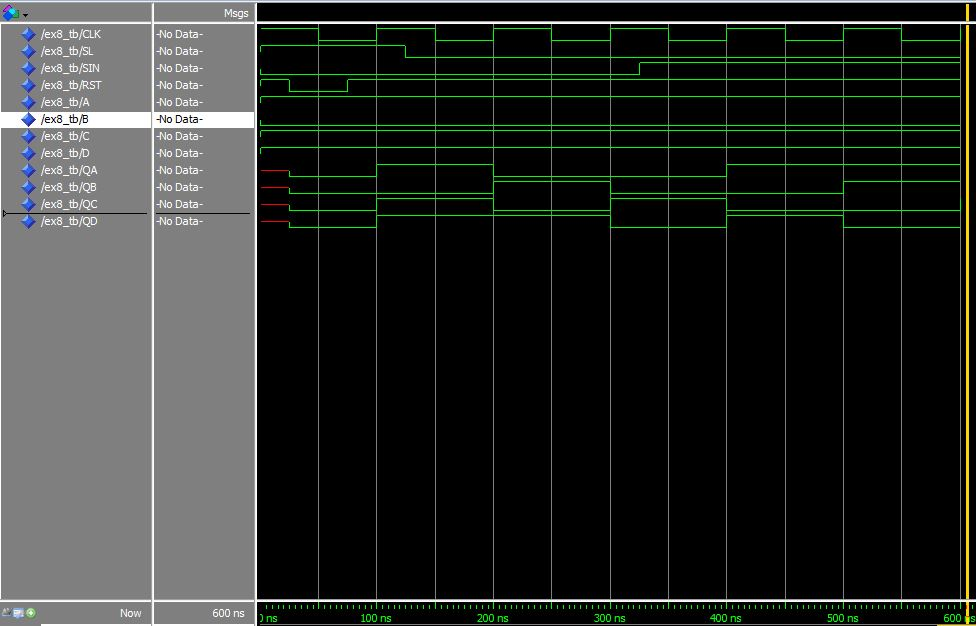
\includegraphics[width=\textwidth]{ModelSim.png}
	\caption{4-bit shift register waveform}
	\label{fig: Figure 3}
\end{figure}

\section*{Conclusion}
The exercise was helpful in understanding the design and operation of sequential circuits, like shift registers. There are multiple ways to design the same sequential circuit as shown by the waveforms of the two shift registers having the same waveforms. The schematic diagrams in the exercise were designed correctly as confirmed by the testbench and the waveform of the diagrams being the same.

\section*{Questions}
1. The arithmetic operation that occurs was division by two without the remainder of the operation.

2.The arithmetic operation that occurs was multiplication by two.

3. It is not a good idea to change the input signals at exactly tthe same time as the rising edge because this creates an unpredictable race-situation which might not work as intended.

\end{document}